\section{Step-by-step example: create and anlalyze synthetic data }
\label{S:EXAMPLESYNTHETICDATA}


This example shows how to create and analyze synthetic data using OpenBDLM.
The objective is to create synthetic time series data with an acceleration stationary baseline, and a yearly periodic pattern as well as a autoregressive process superimposed into it. 
This example corresponds to the OpenBDLM demo presented in Section~\ref{S:OPENBDLMGETTINGSTARTED}

\subsection{Step 1: start a project}

First, choose the interactive tool by typing \colorbox{light-gray}{\lstinline[basicstyle = \mlttfamily \small, backgroundcolor = \color{light-gray}]!0!}.
Secondly, provide a project name (i.e. \lstinline[basicstyle = \mlttfamily \small, backgroundcolor = \color{light-gray}]!SYNTHETIC!).
Then, answer \colorbox{light-gray}{\lstinline[basicstyle = \mlttfamily \small, backgroundcolor = \color{light-gray}]!yes!} to indicate that you would like to create synthetic data.
Finally, type \colorbox{light-gray}{\lstinline[basicstyle = \mlttfamily \small, backgroundcolor = \color{light-gray}]!1!} to create one single synthetic time series. 

\subsection{Step 2: define the time step vector}

Type \colorbox{light-gray}{\lstinline[basicstyle = \mlttfamily \small, backgroundcolor = \color{light-gray}]!2000-01-01!}, \colorbox{light-gray}{\lstinline[basicstyle = \mlttfamily \small, backgroundcolor = \color{light-gray}]!2005-01-01!} and \colorbox{light-gray}{\lstinline[basicstyle = \mlttfamily \small, backgroundcolor = \color{light-gray}]!1!}, to provide the date corresponding of the first and last data sample of the synthetic data, as well as the timestep in days.


\subsection{Step 3: configure the model}

First, the program requests the number of model class.
In this example, we would like to create synthetic data with no anomaly.
In such case, we type \colorbox{light-gray}{\lstinline[basicstyle = \mlttfamily \small, backgroundcolor = \color{light-gray}]!1!} to choose a single model class.
Then, OpenBDLM asks for the type of block component.
As mentionned earlier, the objective is to create synthetic time series data with an acceleration stationary baseline, and a yearly periodic pattern superimposed into it. 
%The presence of a daily periodic pattern is unclear.
Therefore, we choose \colorbox{light-gray}{\lstinline[basicstyle = \mlttfamily \small, backgroundcolor = \color{light-gray}]![13 31 41]!}.
This model considers a trend stationary model with a yearly periodic pattern, and an autoregressive process to be more realistic.
At this time, three figures  that represent the amplitude, timestep and availability of the newly created synthetic data (as shown in Figure~\ref{fig:DataSummaryRaw4}) should popup on the screen.
Type \colorbox{light-gray}{\lstinline[basicstyle = \mlttfamily \small, backgroundcolor = \color{light-gray}]!Q!} to save and quit.

\subsection{Step 4: explore the model}
From the main menu, type  \colorbox{light-gray}{\lstinline[basicstyle = \mlttfamily \small, backgroundcolor = \color{light-gray}]!11!} to see what are the values of model parameters which have been assigned to create the synthetic data.
The model totalizes 6 model parameters, that is 
\begin{gather*}
\bm\theta=\{\sigma_{w, \text{D}}^{LA}, p^{\text{PD1}}_{\text{D}}, \sigma_{w,\text{D}}^{\text{PD1}}, \phi^{AR}_{\text{D}}, \sigma_{w,\text{D}}^{AR}, \sigma_{v,\text{D}}\} 
 \end{gather*}
The default model parameters values are 
\begin{gather*}
\bm\theta^{\text{default}}=\{1\times10^{-8}, 365.24, 0, 0.75, 0.01, 0.01\}, 
\end{gather*}
in agreement with the values indicated in Table~\ref{table:defaultsynthetic}.
Type \colorbox{light-gray}{\lstinline[basicstyle = \mlttfamily \small, backgroundcolor = \color{light-gray}]!R!} to return to the main menu.
Then, type \colorbox{light-gray}{\lstinline[basicstyle = \mlttfamily \small, backgroundcolor = \color{light-gray}]!12!} the see that the default initial hidden states mean, covariance  and model probability values are 
\begin{align*}
 \bm \mu^{1,\text{default}}_{0} & = [	10  -1\times10^{-5}  ,	-0.001	,	10  ,  	10    ,	0         ]^{\intercal}, \text{and} \\
 \text{diag}(\bm\Sigma^{1,\text{default}}_{0})  & = [	0.01  ,	0.01  ,	0.01  	,0.04  ,	0.04  ,	0.01     ], \text{and} \\
 \pi_{0}^{1,\text{default}} & = 1.
\end{align*}
respectively, in agreement with the values indicated in Table~\ref{table:defaultsynthetic}.
Type \colorbox{light-gray}{\lstinline[basicstyle = \mlttfamily \small, backgroundcolor = \color{light-gray}]!R!} to return to the main menu.

\begin{figure*}[h!]
\centering
\begin{subfigure}{\linewidth}
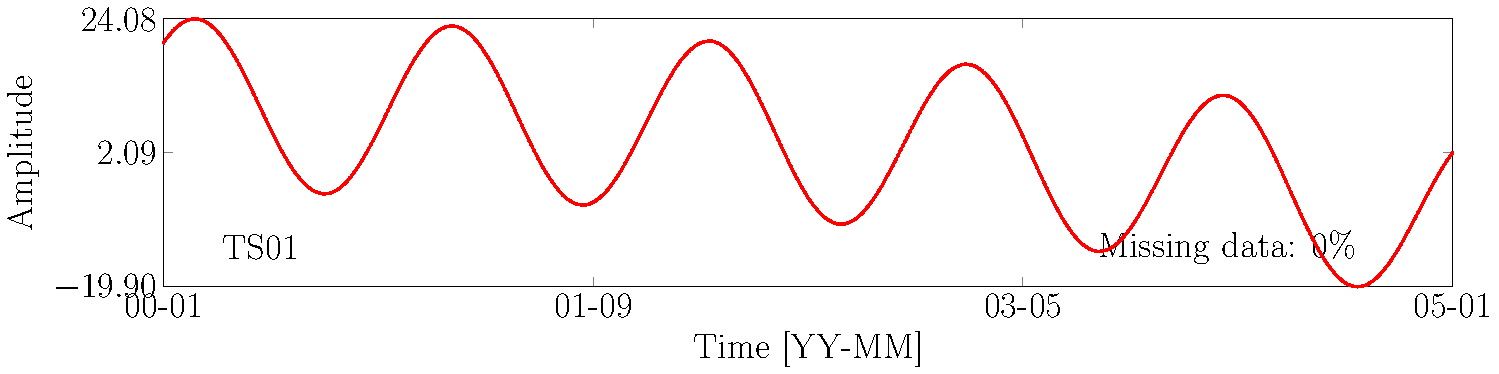
\includegraphics[width=0.9\linewidth]{./docfigs/Example_SYNTHETIC/raw/ALL_AMPLITUDES.pdf} 
\caption{Amplitude}
\end{subfigure}
\begin{subfigure}{\linewidth}
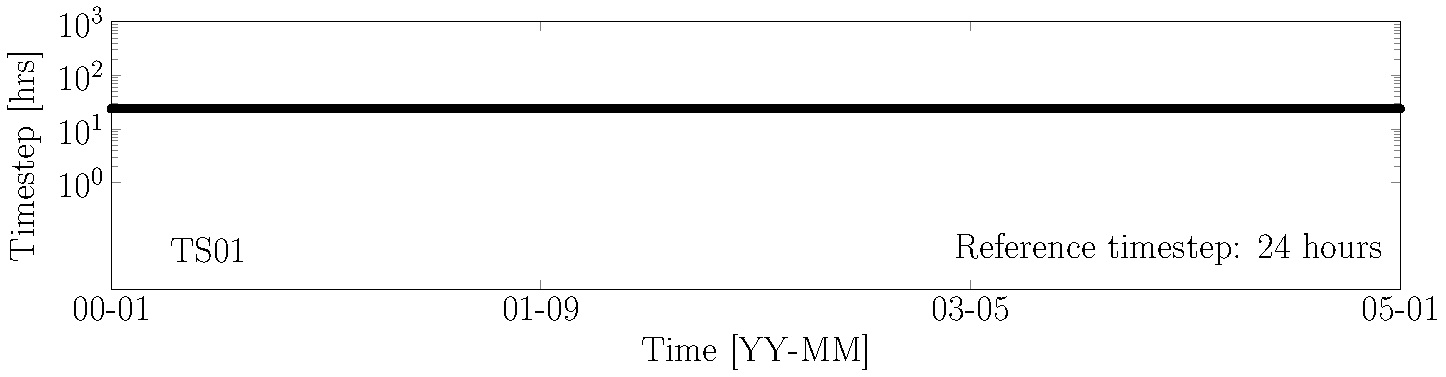
\includegraphics[width=0.9\linewidth]{./docfigs/Example_SYNTHETIC/raw/ALL_TIMESTEPS.pdf}
\caption{Timestep}
\end{subfigure}
\begin{subfigure}{\linewidth}
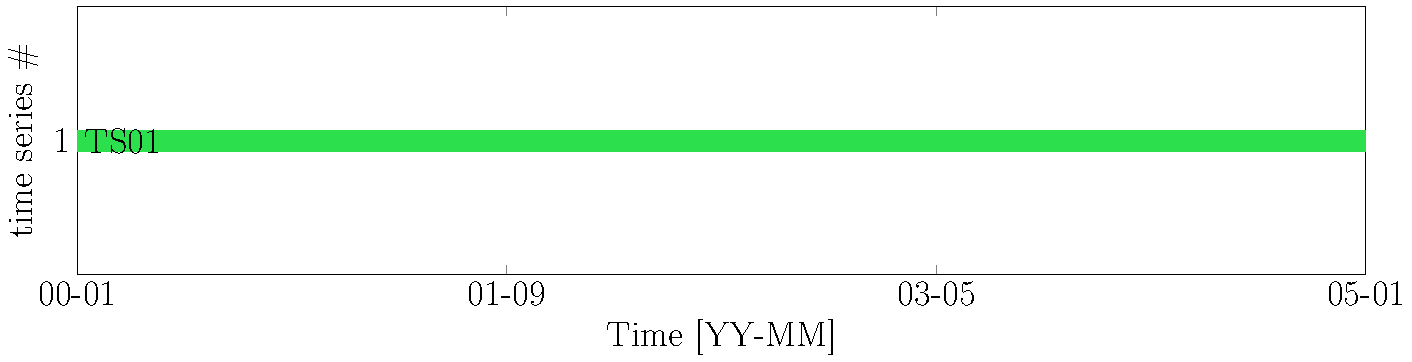
\includegraphics[width=0.9\linewidth]{./docfigs/Example_SYNTHETIC/raw/AVAILABILITY.pdf}
\caption{Availability}
\end{subfigure}
\caption{Data used in Section~\ref{S:EXAMPLESYNTHETICDATA}}.
\label{fig:DataSummaryRaw4}
\end{figure*}


\subsection{Step 5: estimate the hidden states}

From the main menu, type  \colorbox{light-gray}{\lstinline[basicstyle = \mlttfamily \small, backgroundcolor = \color{light-gray}]!3!}, then \colorbox{light-gray}{\lstinline[basicstyle = \mlttfamily \small, backgroundcolor = \color{light-gray}]!1!} to estimate the filtered hidden states using the default model parameters and default initial hidden states values.
The value of the log-likelihood is $4973$, and the estimated hidden states are presented in Figure~\ref{fig:SYNTHETICDefaultDefaultExample4}.
For each figure, the red dashed line represents the true known values of the hidden states.

\begin{figure*}[h!]
\centering
\begin{subfigure}{\linewidth}
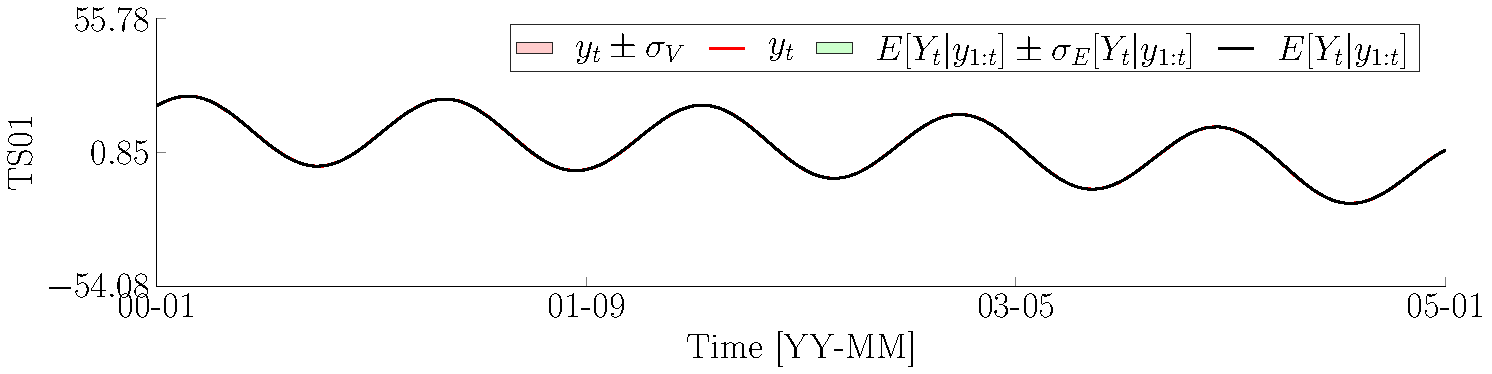
\includegraphics[width=0.9\linewidth]{./docfigs/Example_SYNTHETIC/default/TS01_ObservedPredicted.pdf}
\caption{Observed and estimated displacement data}
\end{subfigure}
\begin{subfigure}{\linewidth}
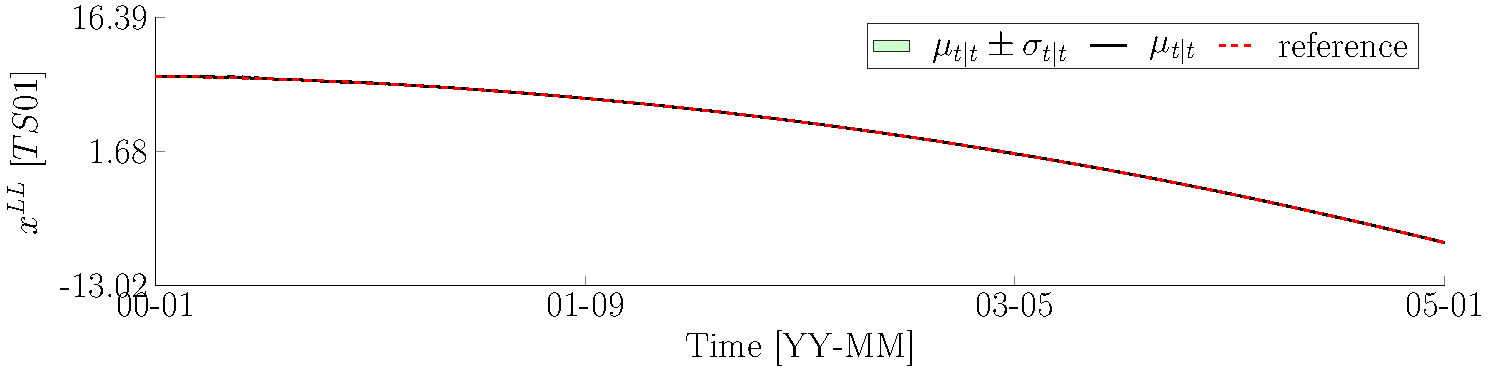
\includegraphics[width=0.9\linewidth]{./docfigs/Example_SYNTHETIC/default/TS01_LL_1.pdf} 
\caption{Estimated displacement local level component}
\end{subfigure}
\begin{subfigure}{\linewidth}
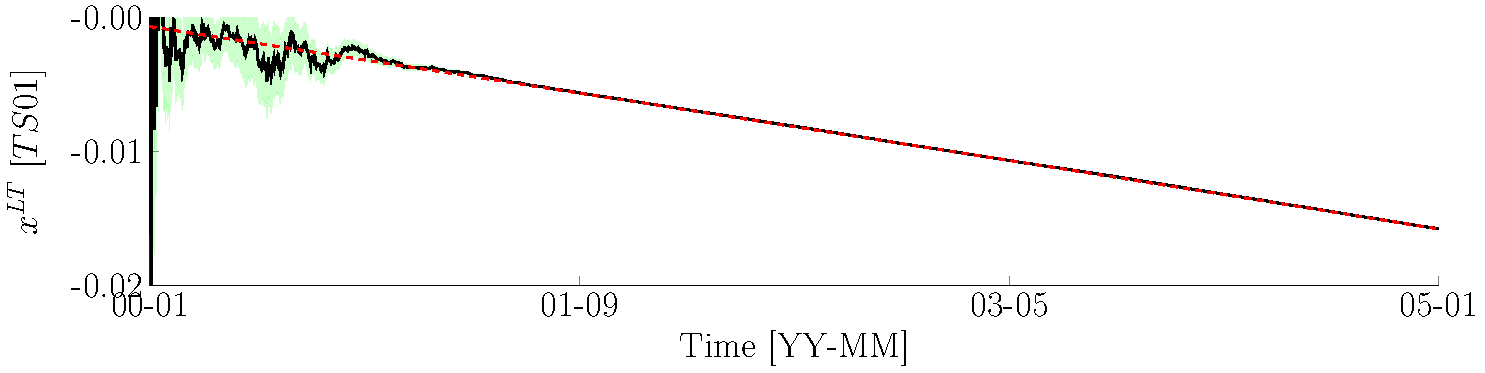
\includegraphics[width=0.9\linewidth]{./docfigs/Example_SYNTHETIC/default/TS01_LT_2.pdf}
\caption{Estimated displacement local trend component.}
\end{subfigure}
\begin{subfigure}{\linewidth}
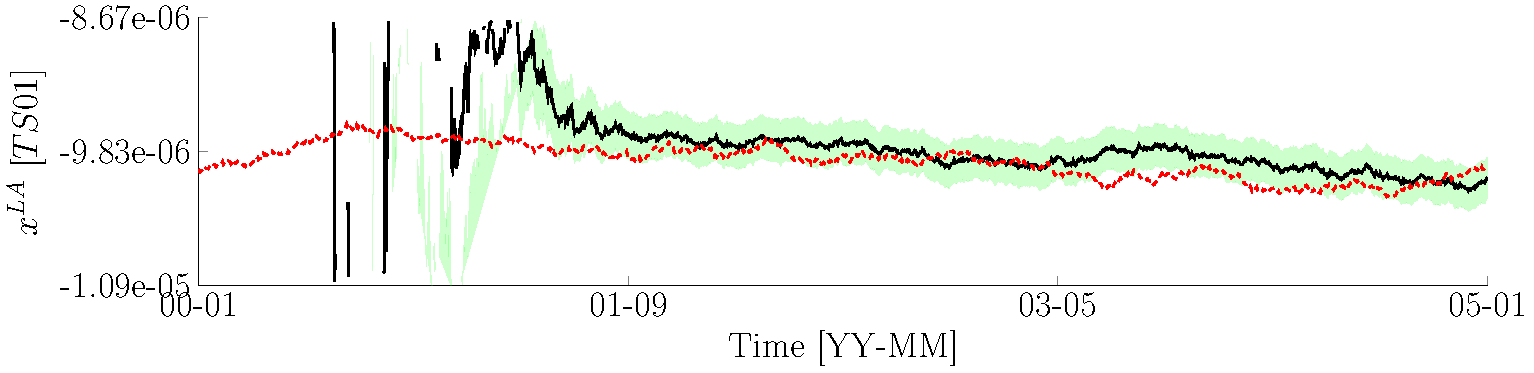
\includegraphics[width=0.9\linewidth]{./docfigs/Example_SYNTHETIC/default/TS01_LA_3.pdf}
\caption{Estimated displacement local acceleration component.}
\end{subfigure}
\end{figure*}
\begin{figure*}[h!]
\ContinuedFloat
\begin{subfigure}{\linewidth}
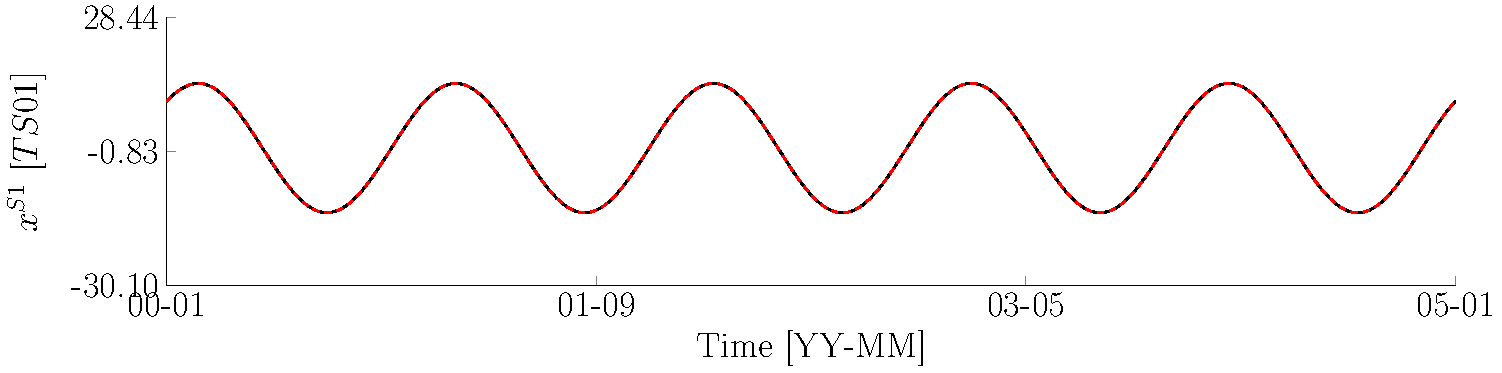
\includegraphics[width=0.9\linewidth]{./docfigs/Example_SYNTHETIC/default/TS01_S1_4.pdf}
\caption{Estimated displacement yearly periodic component (first hidden state)}
\end{subfigure}
\begin{subfigure}{\linewidth}
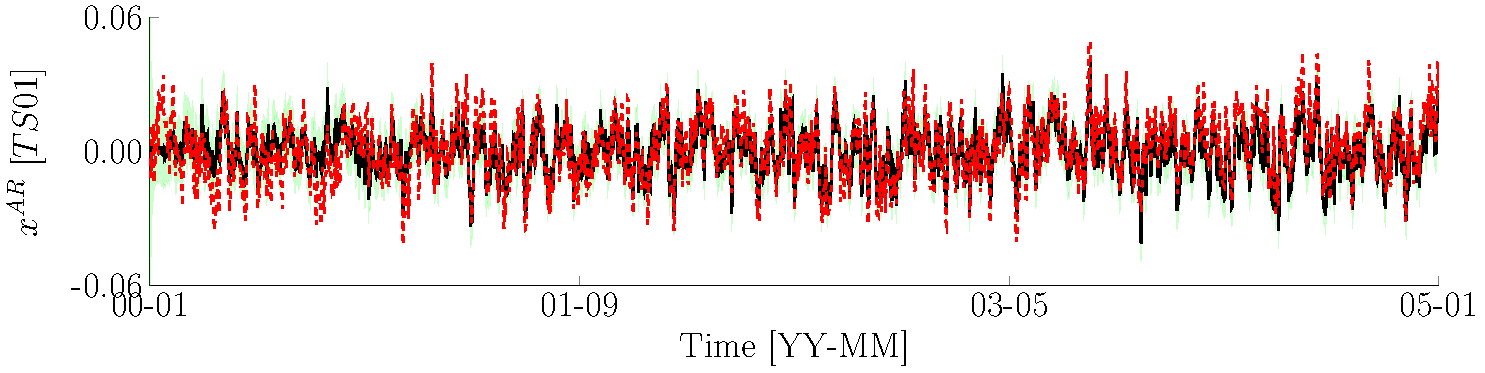
\includegraphics[width=0.9\linewidth]{./docfigs/Example_SYNTHETIC/default/TS01_AR_6.pdf} 
\caption{Estimated displacement autoregressive component}
\end{subfigure}
\caption{Estimated results using OpenBDLM default model parameters and default initial hidden states. The hidden states are estimated from the data presented in Figure~\ref{fig:DataSummaryRaw4}a. The solid line and shaded area represent the mean and standard deviation of the estimated hidden states, respectively. The red dashed line represent the true the hidden state value.}
\label{fig:SYNTHETICDefaultDefaultExample4}
\end{figure*}

\subsection{Step 6: estimate the initial hidden states}

From the main menu, type  \colorbox{light-gray}{\lstinline[basicstyle = \mlttfamily \small, backgroundcolor = \color{light-gray}]!2!}, to optimize the initial hidden states value.
The estimated initial hidden states mean and covariance values are 
\begin{align*}
\bm \mu^{*}_{0} & = [	10 ,   	-0.00103,	-9.68\times10^{-6},	10   , 	10    ,	-0.0106  ]^{\intercal}, \text{and} \\
 \text{diag}(\bm\Sigma^{*}_{0}) & = [	2.35\times10^{-5}	, 1.33\times10^{-9},	3.3\times10^{-14}	, 1.9\times10^{-6}	, 2.03\times10^{-6}	,0.000353    ], 
 \end{align*}
 respectively.
Once it is done, type  \colorbox{light-gray}{\lstinline[basicstyle = \mlttfamily \small, backgroundcolor = \color{light-gray}]!3!}, and then  \colorbox{light-gray}{\lstinline[basicstyle = \mlttfamily \small, backgroundcolor = \color{light-gray}]!1!} to compute the filtered hidden states using the optimized model parameters and optimized initial hidden states.
The value of the log-likelihood is $5008$.
The estimated hidden states are presented in Figure~\ref{fig:SYNTHETICOptimizedOptimizedExample4}.


\begin{figure*}[h!]
\centering
\begin{subfigure}{\linewidth}
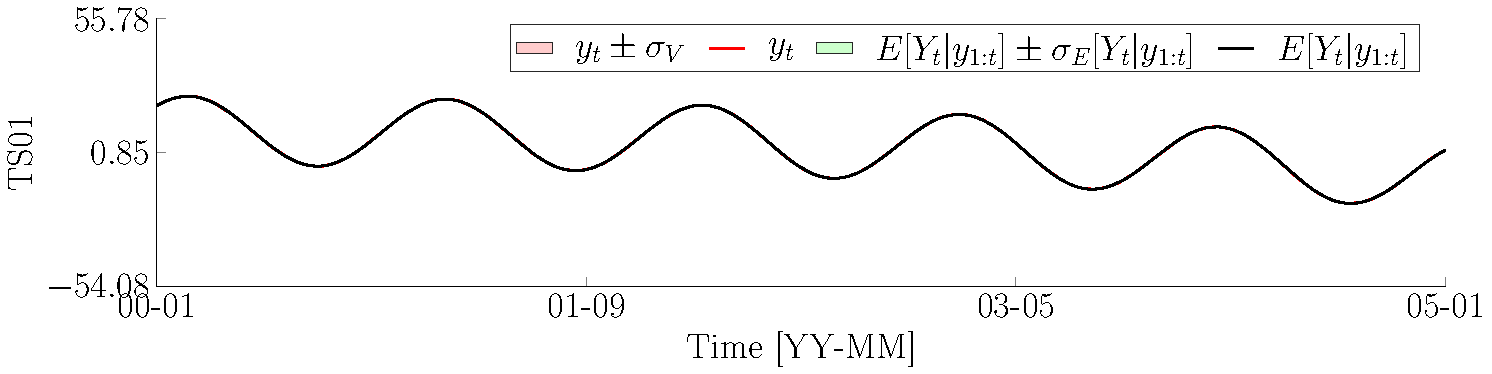
\includegraphics[width=0.9\linewidth]{./docfigs/Example_SYNTHETIC/optim_param_optim_initialhiddenstate/TS01_ObservedPredicted.pdf}
\caption{Observed and estimated displacement data}
\end{subfigure}
\begin{subfigure}{\linewidth}
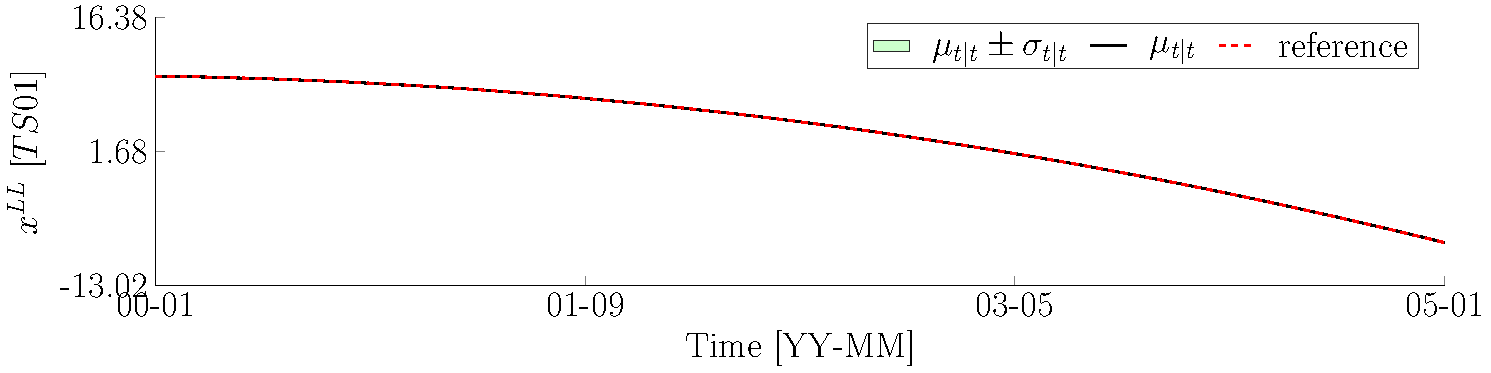
\includegraphics[width=0.9\linewidth]{./docfigs/Example_SYNTHETIC/optim_param_optim_initialhiddenstate/TS01_LL_1.pdf} 
\caption{Estimated displacement local level component}
\end{subfigure}
\begin{subfigure}{\linewidth}
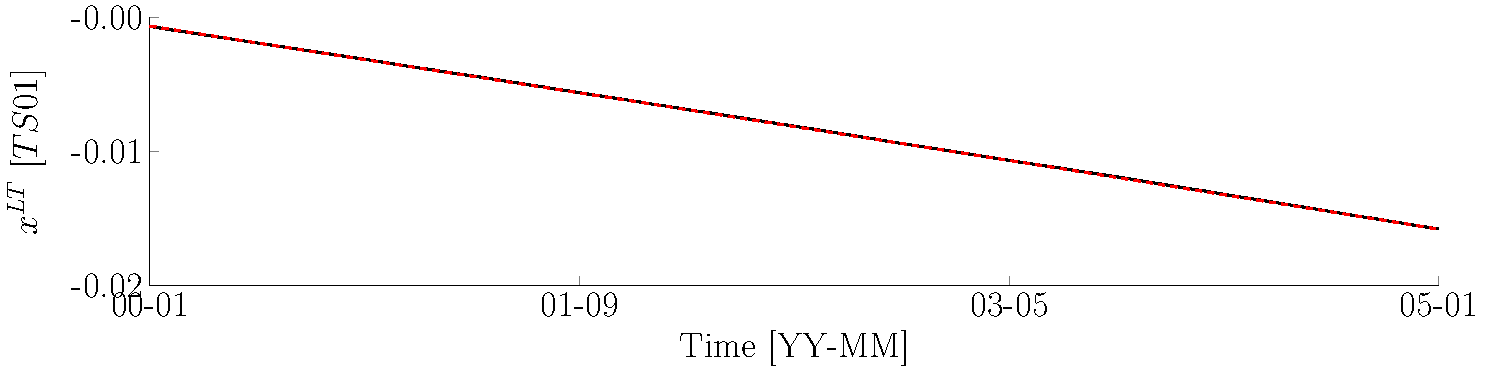
\includegraphics[width=0.9\linewidth]{./docfigs/Example_SYNTHETIC/optim_param_optim_initialhiddenstate/TS01_LT_2.pdf}
\caption{Estimated displacement local trend component.}
\end{subfigure}
\begin{subfigure}{\linewidth}
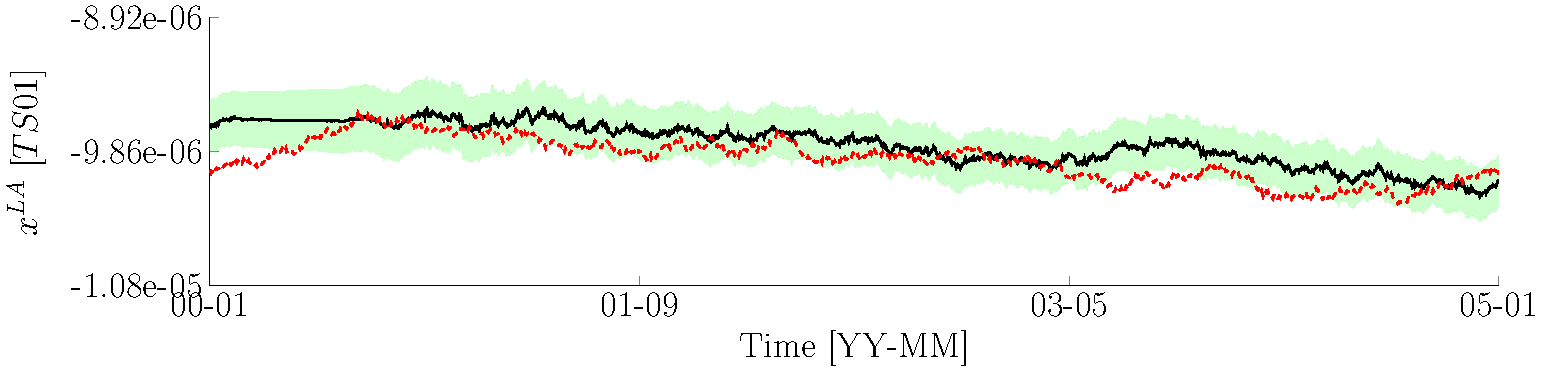
\includegraphics[width=0.9\linewidth]{./docfigs/Example_SYNTHETIC/optim_param_optim_initialhiddenstate/TS01_LA_3.pdf}
\caption{Estimated displacement local acceleration component.}
\end{subfigure}
\end{figure*}
\begin{figure*}[h!]
\ContinuedFloat
\begin{subfigure}{\linewidth}
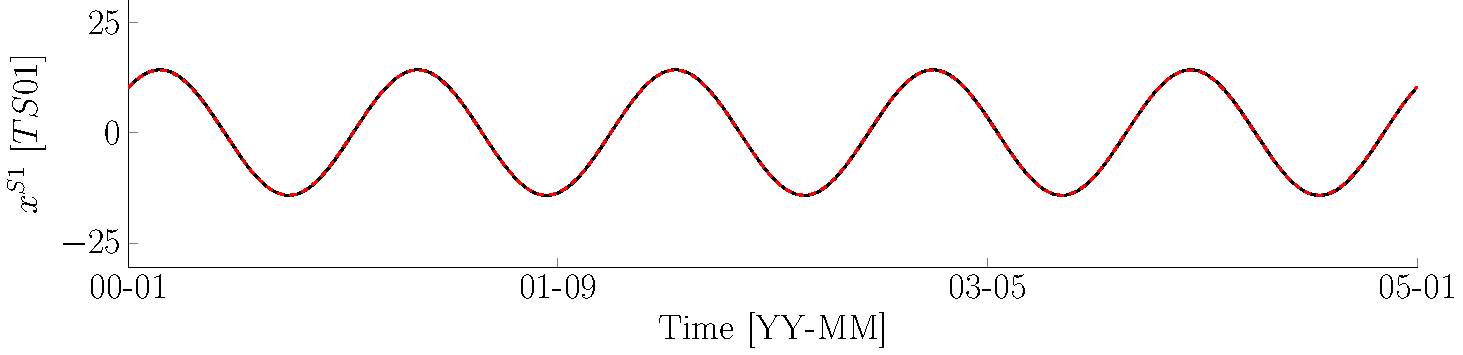
\includegraphics[width=0.9\linewidth]{./docfigs/Example_SYNTHETIC/optim_param_optim_initialhiddenstate/TS01_S1_4.pdf}
\caption{Estimated displacement yearly periodic component (first hidden state)}
\end{subfigure}
\begin{subfigure}{\linewidth}
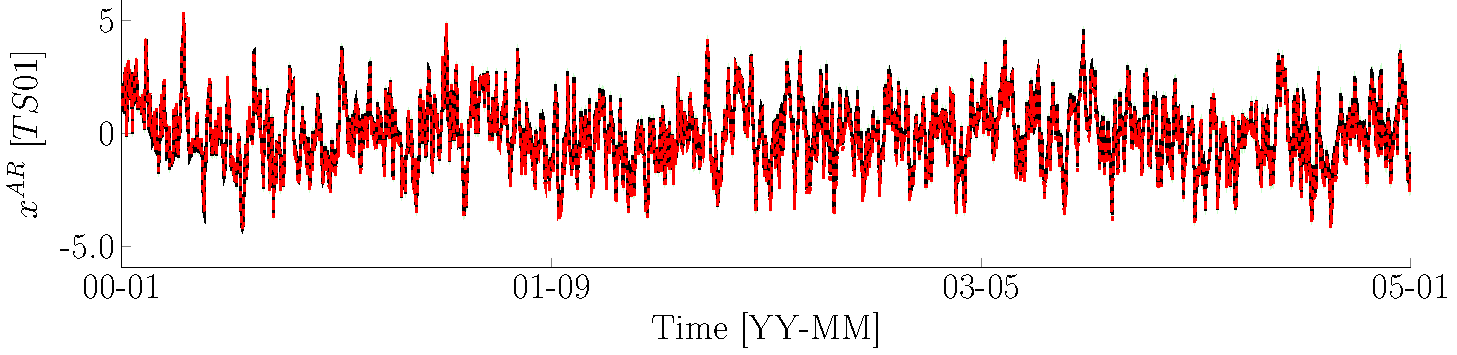
\includegraphics[width=0.9\linewidth]{./docfigs/Example_SYNTHETIC/optim_param_optim_initialhiddenstate/TS01_AR_6.pdf} 
\caption{Estimated displacement autoregressive component}
\end{subfigure}
\caption{Estimated results using OpenBDLM default model parameters and optimized initial hidden states. The hidden states are estimated from the data presented in Figure~\ref{fig:DataSummaryRaw4}a. The solid line and shaded area represent the mean and standard deviation of the estimated hidden states, respectively. The red dashed line represent the true the hidden state value.}
\label{fig:SYNTHETICOptimizedOptimizedExample4}
\end{figure*}


